%%%%%%%%%%%%%%%%
\section{Materials and Methods}\label{sec:intro}
%%%%%%%%%%%%%%%%
Our main contribution is in not using predefined pruning rules.
Instead, we use an objective function which includes the goals that are commonly considered by pruning; in particular maximization of the light intake by removing branches that cause shadowing and removing old and dead branches. This is also combined with the shaping of a tree to take either cylindrical or conical shape. 
The objective function is optimized by using discrete differential evolution method~\cite{kohek_eduapple:_2015}, which is based on the
concept of self-organizing trees of~\cite{palubicki_self-organizing_2009}.


%%%%%%%%%%%%%%%%
\subsection{Tree Growth Model}
%%%%%%%%%%%%%%%%
The tree models used in our approach are represented as a hierarchy of
modules as shown in Fig.~\ref{fig:my_figure1}~a) which is a common approach used in many plant
simulators such as \cite{de_reffye_plant_1988,palubicki_self-organizing_2009,pirk_plastic_2012,prusinkiewicz_development_1988,stava_inverse_2014}. 

The point at which one or more leaves are attached to the stem is called a node and the part of the stem between two nodes is an internode. 
The growth is controlled by apical meristem that is a region of dividing cells that responds by growth against gravity (gravitropism) and
toward the incoming light (phototropism).
Depending on the plant species and environmental factors (light, temperature, nutrients, etc.), the plant produces lateral buds that are either dormant or active, and produces leaves with certain orientation (phylotaxis).
An internode with attached leaves and a lateral bud is called a metamer and a sequence of metamers grown at a single spurt forms a shoot. 
The shoot axis is produced by the terminal bud which is located at the end of the shoot.
\begin{figure}[hbt]
    \centering
    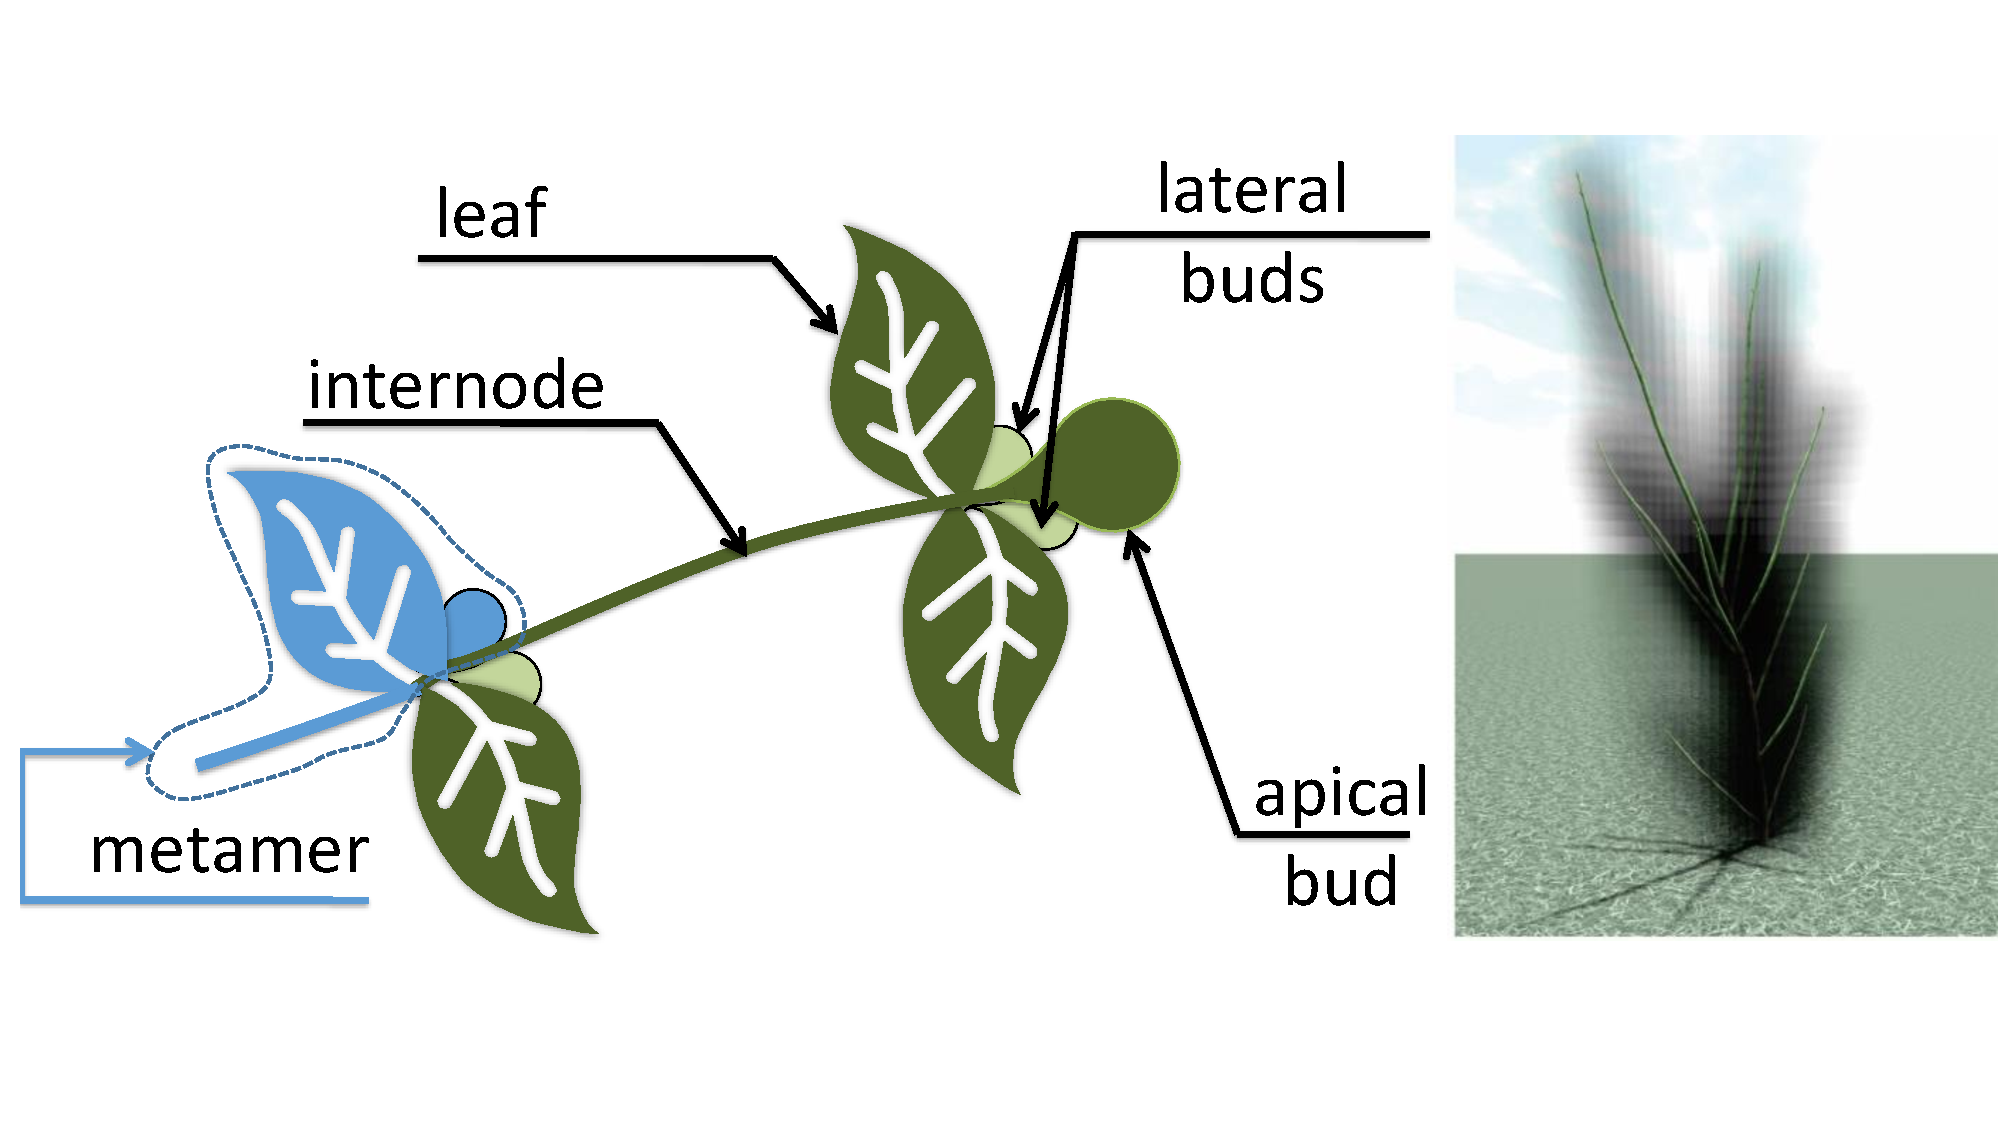
\includegraphics[width=4.5in]{figs/Fig1}
    \caption{a) Plant modules of a self-organizing tree growth
model and b) the shadow space of a tree in used tree growth model from~\cite{kohek_eduapple:_2015}.}
    \label{fig:my_figure1}
\end{figure}

Our approach uses the previously developed framework called EduAPPLE~\cite{kohek_eduapple:_2015},
where a tree growth is driven by buds' illuminations~\cite{benes_efficient_1996,benes_visual_1997,mech_visual_1996} and a competitive process for growth resources~\cite{alsweis_modeling_2005,arvo_modeling_1988,palubicki_self-organizing_2009,runions_modeling_2007}, which leads to the self-organizing structure of the tree. 
The tree attempts to maximize its branch mass by growth and light intake. Buds with higher irradiance produce new shoots that fill
empty space. Buds with lower light intake produce quickly growing shoots
that attempt to get from shade (light seeking stage). Poorly illuminated buds do not create new shoots, become dormant, and can form new shoots later, when the conditions are more favorable. The key factor of this simulation is the calculation of the illumination of leaves that feed buds. Although inner reflection can be considered~\cite{soler_efficient_2003},
the algorithms are usually time consuming, and the indirect light does
not contribute significantly to growth, because major light intake is
given by the direct lighting. A faster way is to use only the direct
irradiance~\cite{benes_efficient_1996,benes_visual_1997,mech_visual_1996,pirk_plastic_2012}. 

The tree cast shadow on itself and thus
forming a shadow space of the tree as shown in Fig.~\ref{fig:my_figure1}~b). The shadow
density is highest at the trunk; thus leaves/shoots rarely grow from the
dormant buds positioned there. Trees produce shoots on their trunks rarely (for example when they are sick), because of the low lighting, thick bark, etc. This is in tune with observations in Nature~\cite{wohlleben2016hidden}.



%%%%%%%%%%%%%%%%%%%
\subsection{Illumination}
%%%%%%%%%%%%%%%%%%
The key contribution of pruning is in
improving the illumination of the inner parts of the tree. When the
lighting conditions around the stem improve after removing some
branches, dormant buds can reactivate and start to produce new shoots. We calculated the inner shading by using the algorithm from~\cite{palubicki_self-organizing_2009}
that was later extended in~\cite{pirk_plastic_2012,stava_inverse_2014,strnad_novel_2017}. 

The light distribution
inside the tree crown is calculated from the illuminated buds that are
sources of a conical shadow volume. We calculate the bud illumination.
Assume a bud inside one of the shadow volumes of one of the
neighbors. Let \(d_{y}\) be the bud's vertical distance from the volume
apex and \(d_{x,z}\) its horizontal distance from the volume axis, then
the received shadow, originating from a given shadow volume is
calculated by~\cite{strnad_novel_2017}:
\begin{equation}
\Delta s = \left\{ \begin{matrix}
\text{ab}^{- 0.8\left( d_{y} + d_{x,z} \right)}, & \mathrm{\text{if}}\ d_{x,z} < d_{y} \\
0, & \mathrm{otherwise} \\
\end{matrix}, \right.\    
\end{equation}
where \(a\) \textgreater{} 0 and \(b\)\textgreater{} 0 are model
parameters from \cite{palubicki_self-organizing_2009} and were set to \(a = 0.05\) and \(b = 2\).
Total irradiance $Q$ of a given bud is then
\begin{equation}
  Q = max\{1 - s, 0\}\label{eqn:q}  
\end{equation}
where \(s\) is the cumulative contribution of all shadow volumes,
captured by the given bud.

%%%%%%%%%%%%%%%%%%
\subsection{Differential Evolution and Pruning}
%%%%%%%%%%%%%%%%%%
The Differential Evolution (DE) is a heuristic approach for minimizing possibly nonlinear and non-differential continuous objective function. Developed by Storm and Price~\cite{storn_differential_1997}, the method aims to optimize certain properties of a system pertinently choosing the system parameters, usually represented as a vector. 

An objective function models the goals, while incorporating potential constraints. For the objective function 
\begin{equation}
f:X \subseteq\!R^{n}\rightarrow \!R,
\end{equation}
where $X\neq\emptyset$, the minimization problem is to find solution vector $\mathbf{s}\in X$, such that $f(\mathbf{s})\leq f(\mathbf{p}), \forall \mathbf{p}\in X$. 
Inspired by genetic algorithms~\cite{davis1991handbook}, DE employs evolutionary operators like mutation, crossover, and selection, to minimize the objective function. The three operators are sequentially (in a fixed order) carried out in a loop, until an adequate fitness or number of iterations is reached.

The DE produces a population of individuals and evaluates their fitness function (light intake in our case). The \textbf{mutation operator} produces a trial vector for each individual of the current population by mutating a target vector with a weighted differential. 
For each parent $\mathbf{x}_{i}\in X$ three distinct individuals $\mathbf{x}_{i_1}$,  $\mathbf{x}_{i_2}$, and $\mathbf{x}_{i_3}$ are selected randomly from the population, $i \neq i_1 \neq i_2 \neq i_3$ and used to calculate the trial vector $\mathbf{u}_i$ as follows:
\begin{equation}
    \mathbf{u}_i = \mathbf{x}_{i_1}+\beta\times (\mathbf{x}_{i_2}-\mathbf{x}_{i_3})
\end{equation}
where $\beta \in (0, \infty )$ is called the differential weight. Together with the population $\beta$ can greatly impact the optimization performance. Both parameters, the differential weight and population size are selected by the user.

The DE  \textbf{crossover operator} implements a discrete recombination of trial $\mathbf{u}_i$ and the parent $\mathbf{x}_i$ vectors, to produce offspring $\mathbf{x}^{,}_i$. The crossover operator is defined by ~\cite{engelbrecht2008computational}:
\begin{equation}
     x^{,}_{i,j} = \ \left\{ \begin{matrix}
u_{i,j}, & \mathrm{\text{if}}\ j \in C \\
x_{i,j}, & \mathrm{\text{otherwise}} \\
\end{matrix} \right.\   
\end{equation}
where $x^{,}_{i,j}$ refers to the $j$-th element of the vector $\mathbf{x}_i$ and $C$ is the set of randomly selected crossover points.

The \textbf{Selection operator} is then applied to construct the population for the next generation. The offspring replaces the parent if the fitness of the offspring surpasses that of the parent otherwise the parent survives to the next generation. This ensures that the average fitness of the population does not deteriorate.

%%%%%%%%%%%%%%%%%%%%%%%%%
\subsubsection{Discrete Differential Evolution}
%%%%%%%%%%%%%%%%%%%%%%%%%
Discrete DE (DDE) variants have been presented in relation to specific
combinatorial optimization problems, e.g., \cite{davendra_flow_2009,pan_discrete_2008,wang_novel_2010}. 

DDE has
been used for the optimization of light condition inside the tree crown
by removing certain branches in \cite{strnad_novel_2017}.
Through optimization of pruning locations, a combination of cuts is obtained
that maximizes the amount of light received by the remaining buds of the
tree crown. For that purpose, for all buds in the tree crown the
irradiance is calculated by the use of Eq. (\ref{eqn:q}). A bud's irradiance, \(Q\)
corresponds to the percentage of available light intercepted by the bud.
For the sake of faster detection of ancestor/successor relationship
between internodes, each internode is associated with a unique
variable-length binary string as shown in~Fig.~\ref{fig:my_figure2}. 

Tree crown light
distribution is calculated next, where the irradiance of each bud in the crown is assigned to one of ten quantization classes of equal width of $0.1$ on
the interval $[0, 1]$. The objective function 
\emph{f}(\textbf{x}) is:
\begin{equation}
 f\left( \mathbf{x} \right) = \frac{\sqrt{S_{\mathrm{\text{tree}}}}}{H}\sum_{i = 1}^{10}{i \times h_{i}}, 
\end{equation}
where \(S_{\mathrm{\text{tree}}}\) is the number of remaining internodes
after pruning, \emph{H} is the total number of buds, and \(h_{i}\) is
the number of buds in the \emph{i}-th class of light distribution.

The solution vector is denoted by
\(\mathbf{x} = \ \left\{ x_{1},\ \ldots,x_{s} \right\}\) and it contains
the encoded sequence of cut positions, labeled by the corresponding
internodes. The root is denoted by a bit-string ``0''. A `0' or `1' is
appended to the parent's string for each main or lateral child
internode, respectively (Fig.~\ref{fig:my_figure2}). Each cut position \(x_{i}\)
identifies the internode, at which the branch is removed. Variable
\emph{s} in this case is a population size and is a value between
\(s_{\mathrm{\min}}\) and \(s_{\mathrm{\max}}\), which are custom set
parameters, representing the minimum and the maximum number of allowed
cuts. The objective function \(f(\mathbf{x})\) favors solutions that
provide a maximal improvement of light distribution with a minimal amount
of removed biomass. It is important to recognize and ignore redundant cuts,
for example, if a cut should be made at internode ``00'', the cuts
``001'', ``000'', or ``0010'', would be redundant and thus unnecessary
as shown in Fig.~\ref{fig:my_figure2}. Our labeling allows for quick detection of the
redundant cuts. In a given example the later three internodes share the
same prefix ``00'', which is the label of their predecessor and with
removing it, all of its successors are removed as well.
\begin{figure}[hbt]
    \centering
    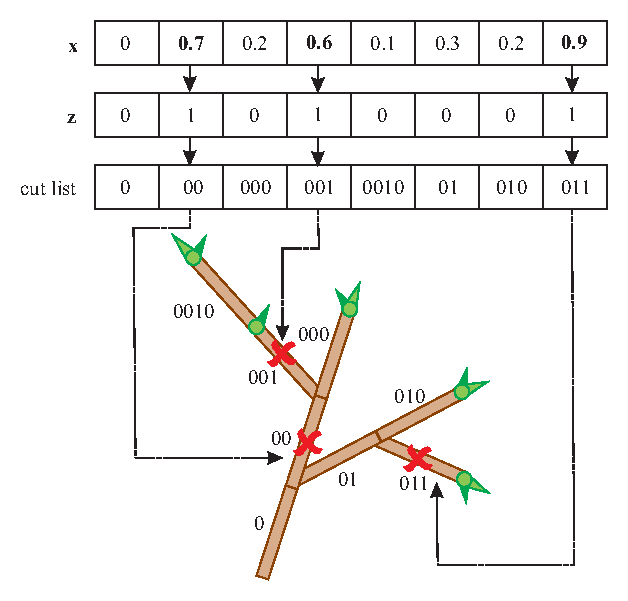
\includegraphics[width=3.3in]{figs/Fig2.pdf}
    \caption{Mapping of the solution vertex into the tree cutting
sequence - genotype to fenotype mapping. Solution vector components that exceed the threshold are converted into the cuts with the help of the cut list.}
    \label{fig:my_figure2}
\end{figure}

The encoding scheme uses the real-valued vectors to
represent solution genotypes as shown in Fig.~\ref{fig:my_figure2}. 
For the mapping of genotypes to fenotypes (i.e. pruning
instances), the intermediate cut list is used. It is produced by
traveling the tree model in a depth-first manner and recording the
labels of all internodes encountered in the process into a list. The
length of the cut list defines the dimensions of solution vectors. Each
component \(x_{i,j} \in \ \left\lbrack 0,\ 1 \right\rbrack\) of the
solution vector \(\mathbf{x}_{i}\ \)determines whether \emph{j}-th
internode from the cut list will be selected as the cutting point or
not. For that purpose the binary vector \(\mathbf{z}_{i}\) is
constructed by thresholding:
\begin{equation}
    z_{i,j} = \ \left\{ \begin{matrix}
0, & \mathrm{\text{if}}\ x_{i,j} < 0.5 \\
1, & \mathrm{\text{otherwise.}} \\
\end{matrix} \right.\
\end{equation}

If the number of cuts proposed by the vector \(\mathbf{z}_{i}\) violates
the solution size constraints, the threshold is adjusted up or down
until the constraints are met. 

\subsection{Tree Height and Neighboring Distance Control}
Although the DDE method improves the light conditions
inside the tree crown, it offers no control over the tree size or the
distance to neighbor trees. Since the modern orchards are mostly
protected by the anti-hail nets, it is crucial to keep apple trees below the
certain height. Similarly, the neighboring distance has to be
preserved during the entire lifetime of an orchard so that the tree branches do not overlap and do not compete for the same space.

A straightforward method to get control over the tree height and
neighboring distance would be the extension of the objective function
\(f\left( \mathbf{x} \right)\) with additional constraints regarding the
tree size. It turned out, however, that while the integration of the
tree height into the tree model and objective function is possible, the
determination of the extent of the tree crown after the pruning was not
efficient, since the buds' locations inside the tree have to be included into the growth model for that purpose. This would lead to higher memory requirements and increased processing time.

Our inspiration for the solution to this problem comes from observing a
human during manual pruning. Instead of just following the pruning
rules, the human pruner strives to shape the tree into one of the
well-defined growing forms. Those growing forms were developed over the
years by the experts and gave the best fruiting results under certain
growing conditions. In high density orchards, the most common tree
forms are the Slender Spindle~\cite{weber_optimizing_2000}, and more recent, the Tall
Spindle~\cite{robinson_vision_2013}. While the Slender Spindle is conically shaped, see Fig. \ref{fig:my_figure2a}a,
the Tall Spindle resembles a cylinder (Fig. \ref{fig:my_figure2a}b). Tall spindle is very popular because it
is suitable for mechanical pruning and formation of the Fruiting Wall~\cite{robinson_vision_2013}.

\begin{figure}[hbt]
    \centering
    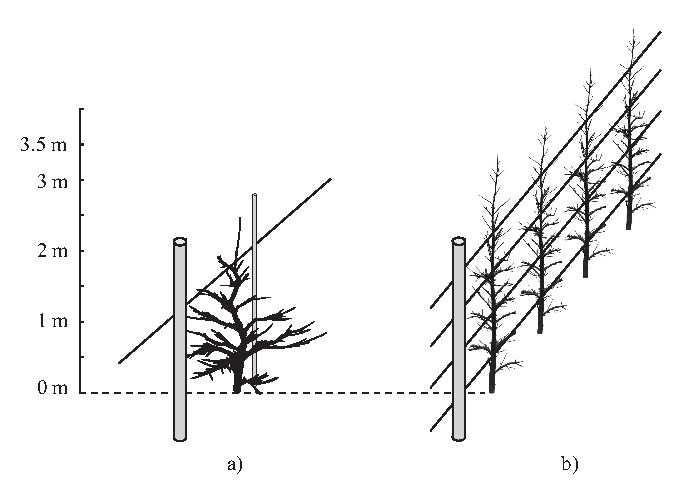
\includegraphics[width=4.2in]{figs/Fig3.pdf}
    \caption{High density apple systems a) Slender Spinle is a growing form used in older orchards, b) Tall Spindle is a recent growing form with higher yields.}
    \label{fig:my_figure2a}
\end{figure}

Instead of changing the objective function, we propose adding a
preprocessing level to the DDE method. We call this step Shaping  and
by adding this the desired form, the tree height and neighboring
distance can be controlled easily. We prune the trees to either a conical or a cylindrical shape
with adjustable height and the base radius. After
the branches outside the chosen shape are trimmed off, the DDE method is
used to optimize the light condition inside the tree crown. The entire
tree pruning process is depicted in Fig.~\ref{fig:my_figure3}.
\begin{figure}[hbt]
    \centering
    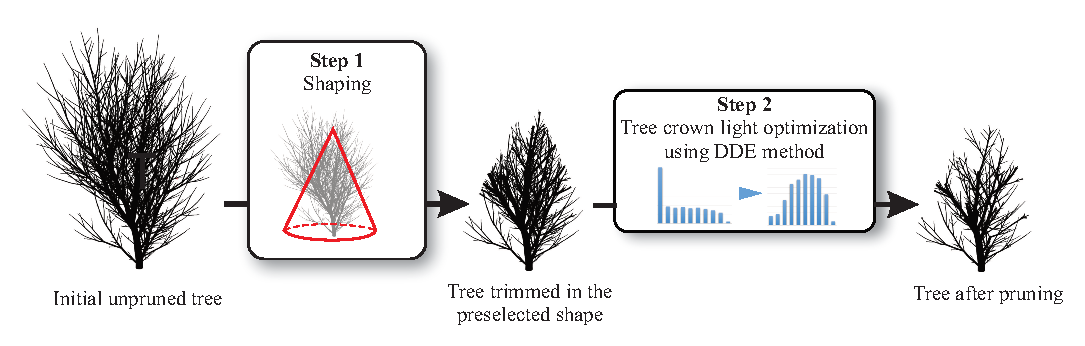
\includegraphics[width=5.3in]{figs/Fig4.pdf}
    \caption{Two-step virtual pruning process enables the control
over tree height and neighboring distance. First, the tree is shaped
into a cone or cylinder shape with adjustable size. In the second step
the DDE method selectively removes branches to improve the light
conditions inside the tree crown.}
    \label{fig:my_figure3}
\end{figure}

The results of the final pruning depend on the maximum
allowed number of cuts \(s_{\mathrm{\max}}\), which has to be adjusted
to the tree age and thus complexity of the tree crown. In our implementation,
we set \(s_{\mathrm{\max}} = 20\) which provided good results for young
trees. 

While we used circular proxies in our work, other shapes could be
used: for example, orchards with Fruiting Wall planting system could use
rectangular blocks.
